% Created 2017-03-01 Wed 20:38
\documentclass[10pt]{article}
\usepackage[utf8]{inputenc}
\usepackage[T1]{fontenc}
\usepackage{fixltx2e}
\usepackage{graphicx}
\usepackage{longtable}
\usepackage{float}
\usepackage{wrapfig}
\usepackage{rotating}
\usepackage[normalem]{ulem}
\usepackage{amsmath}
\usepackage{textcomp}
\usepackage{marvosym}
\usepackage{wasysym}
\usepackage{amssymb}
\tolerance=1000
\usepackage{natbib}
\usepackage[linktocpage,pdfstartview=FitH,colorlinks,
linkcolor=blue,anchorcolor=blue,
citecolor=blue,filecolor=blue,menucolor=blue,urlcolor=blue]{hyperref}
\usepackage[margin=2cm]{geometry}
\pagenumbering{gobble}
\usepackage{wrapfig}
\usepackage{multicol}
\setlength\columnsep{20pt}
\author{Alejandro Rodríguez Salamanca: r0650814@student.kuleuven.be}
\date{}
\title{Artificial Neural Networks: Session 2}
\begin{document}

\maketitle
\begin{multicols}{2}

\section*{Exercise 1}

\subsection*{Hopfield network}

In this first exercise, a Hopfield network is created with attractor states in the corners of the plot. 
Starting with an initial random position, it reaches one of the attractors as it is expected.

\begin{center}
	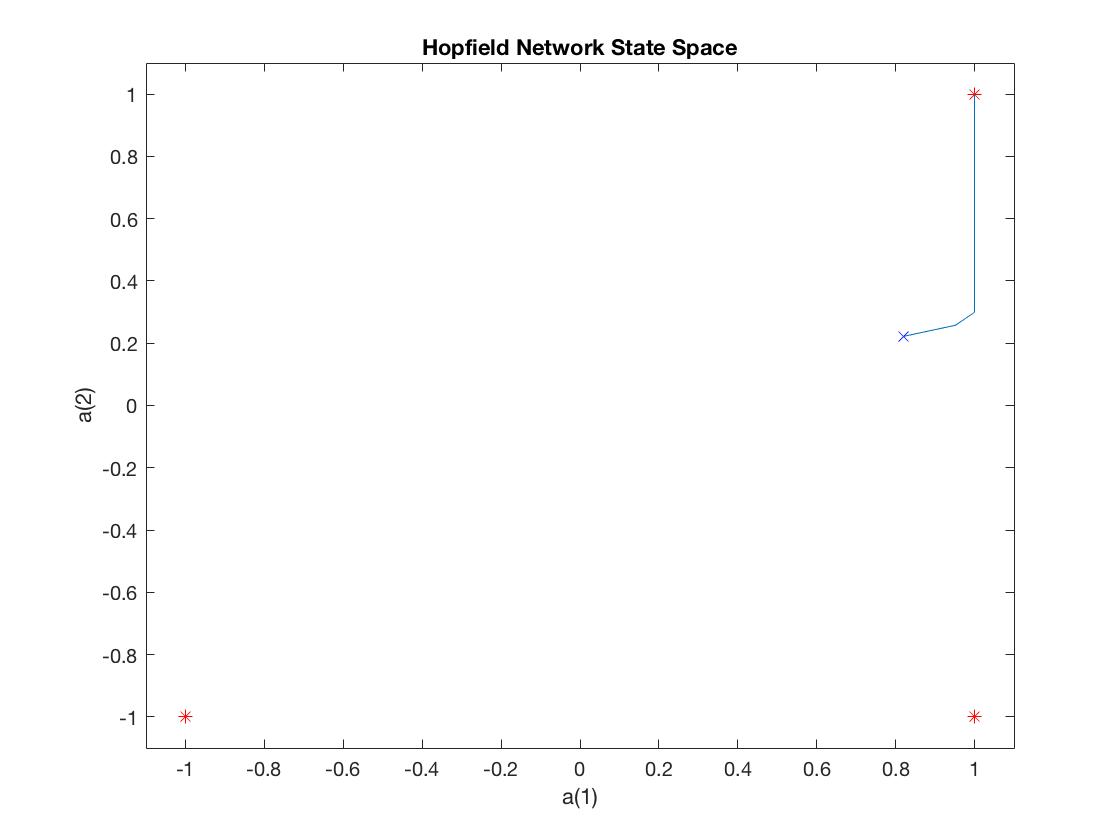
\includegraphics[width=0.8\linewidth]{img/stable1}
\end{center}

But after performing several experiments, we realise that other attractor states also exists. This states can
be seen in the following plot. It is initialised with eight different points choosen carefully to show that 
in the upper left corner there is also another attractor state.

Moreover, the points (0, -1), (1, 0), (0, 1), (-1, 0) can be also considered attractor states.
If we look at this points in the following figure, our initial vectors get stuck there.
This is because this points are in the middle of two attractor points. For this reason, they can be considered a local minimum.

\begin{center}
	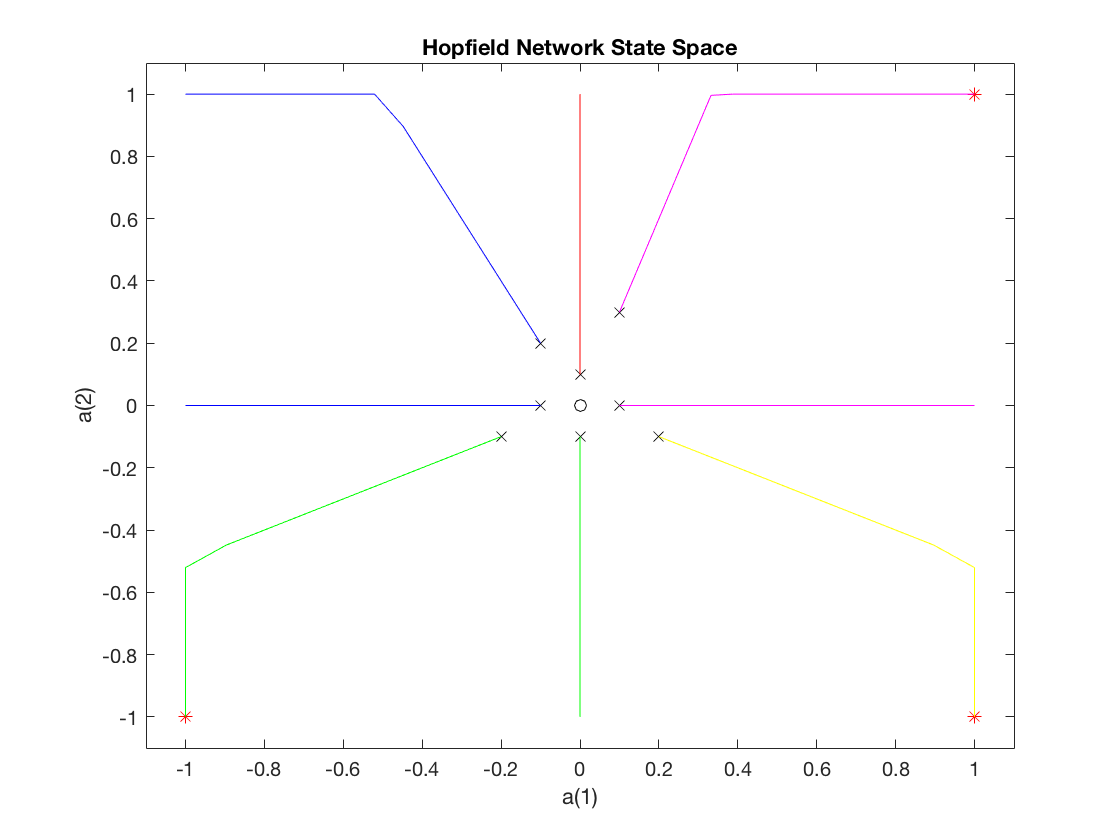
\includegraphics[width=0.8\linewidth]{img/stable2}
\end{center}

\subsection*{rep2 and rep3}

For this exercise the initialisation of the points has been changed from random, to a fixed vector of high 
symmetry points, \texttt{P}. This points are the ones used in the previous exercise, so we can expect to obtain the same results.

\begin{verbatim}
P = [-0.2 -0.1 +0.1 +0.2 +0.0 +0.0 -0.1 +0.1;  
     -0.1 +0.2 +0.3 -0.1 +0.1 -0.1 +0.0 +0.0];
\end{verbatim}

In the next figure it can be seen that this network contains more attractor states that the ones defined at
the creation. The reason has already been explained in the previous exercise.

\begin{center}
	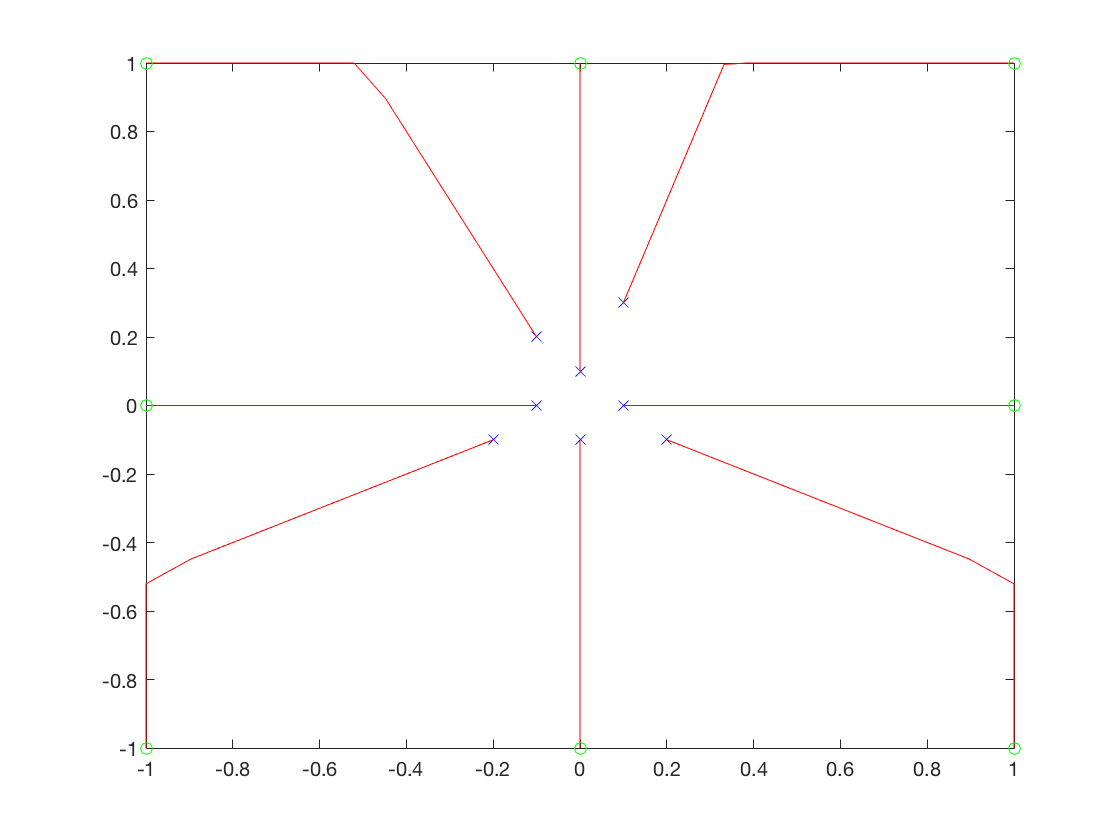
\includegraphics[width=0.8\linewidth]{img/rep2}
\end{center}

In the case of \texttt{rep3}, we have follow another approach. Here, a hundred random points have been created,
and the network has perfom 50 iterations. After that, the following plot has been obtained.

In this plot we can see that all the points converge into an attractor state.
Unlike in \texttt{rep2}, it can be determined that the attractor states are the ones defined when the network is created.

\begin{center}
	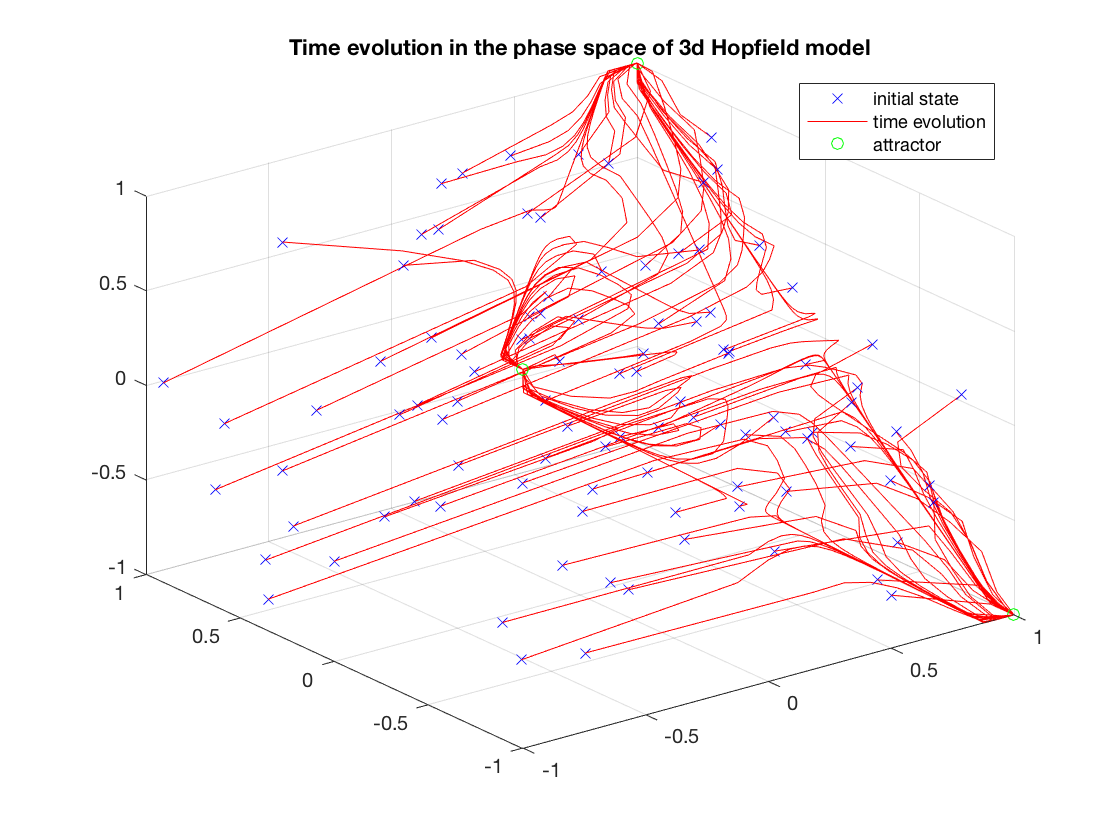
\includegraphics[width=0.8\linewidth]{img/rep3}
\end{center}

\subsection*{hopdigit}

Executing \texttt{hopdigit\_v2(1,10)}, where \texttt{noise} equals 1, and \texttt{numiter} equals 10, the following result is obtained.

\begin{center}
	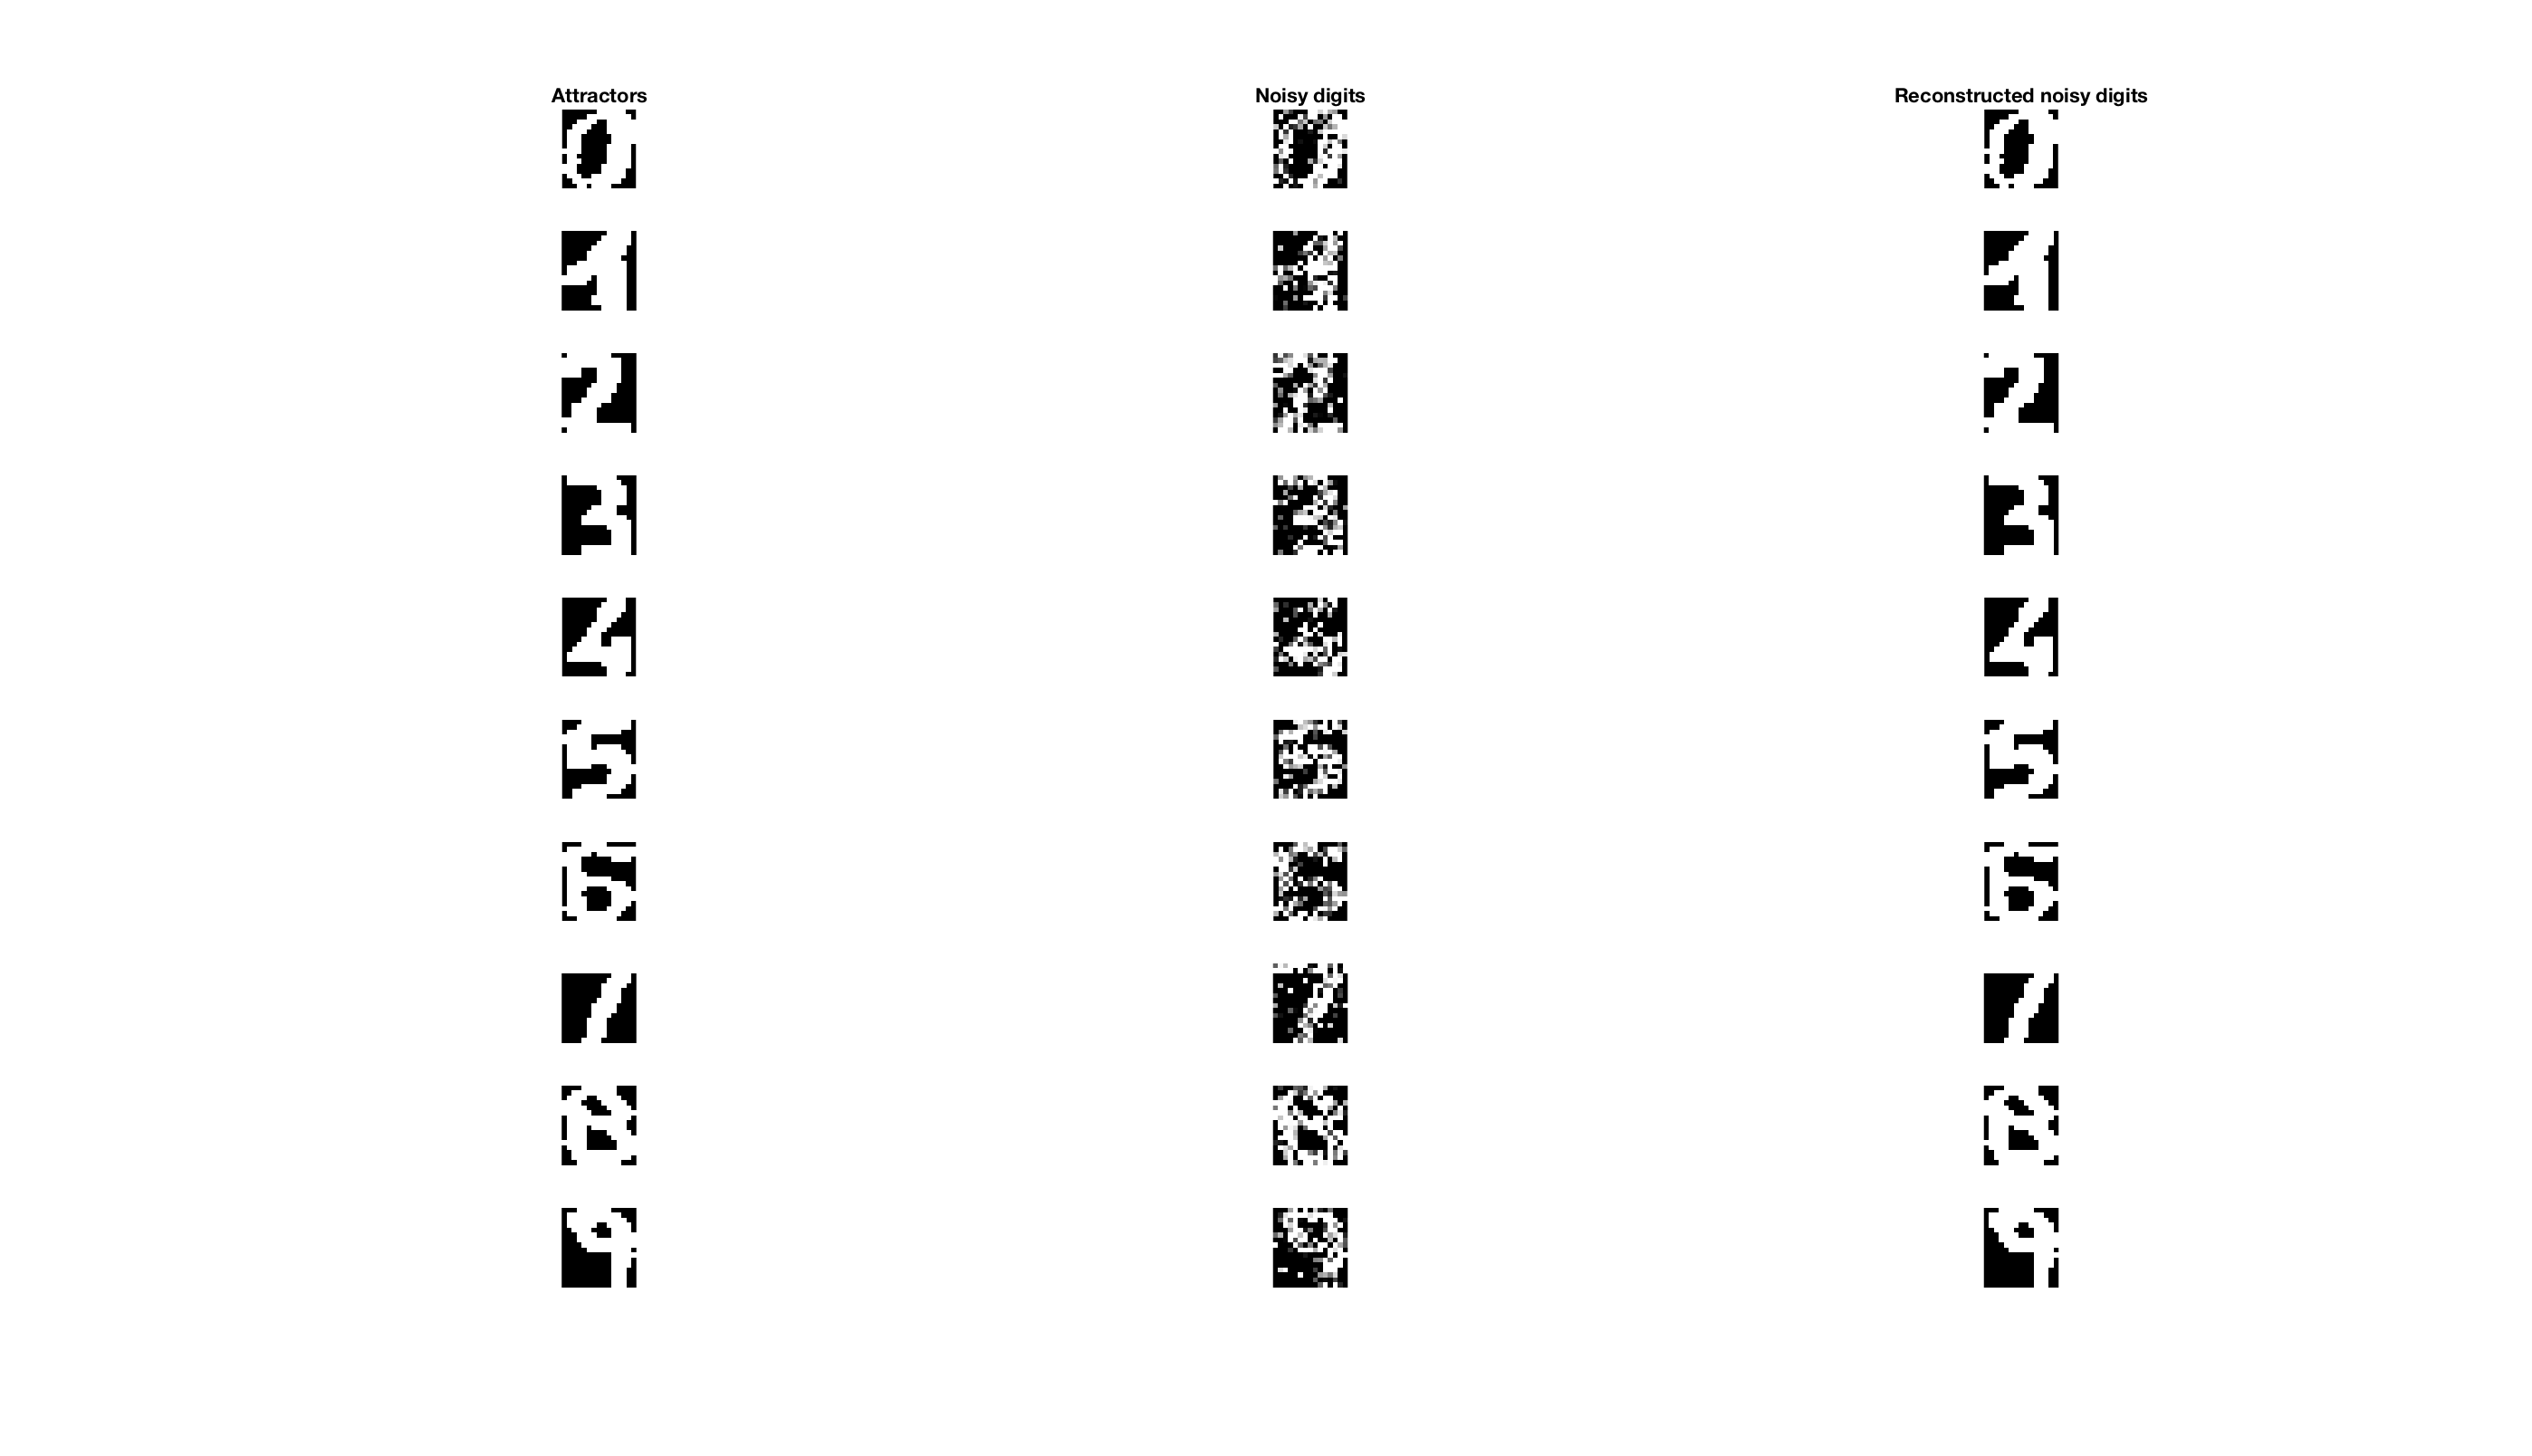
\includegraphics[width=0.8\linewidth]{img/hop1-10}
\end{center}

The left column corresponds with the original handwritten numbers, the middle column contains this digits with noise,
and the right column shows the digits retrieved by the neural network.

After adding some more noise to the digits, it is possible to appreciate the efectiveness of the neural network to
identify digits.

Moreover, playing with the number of iterations and the noise at the same time shows that a higher
number of iterations does not mean a higher accuracy. In the next two pictures the results of \texttt{noise = 5, iterations = 90}
and \texttt{noise = 6, iterations = 10} are shown.

\begin{center}
	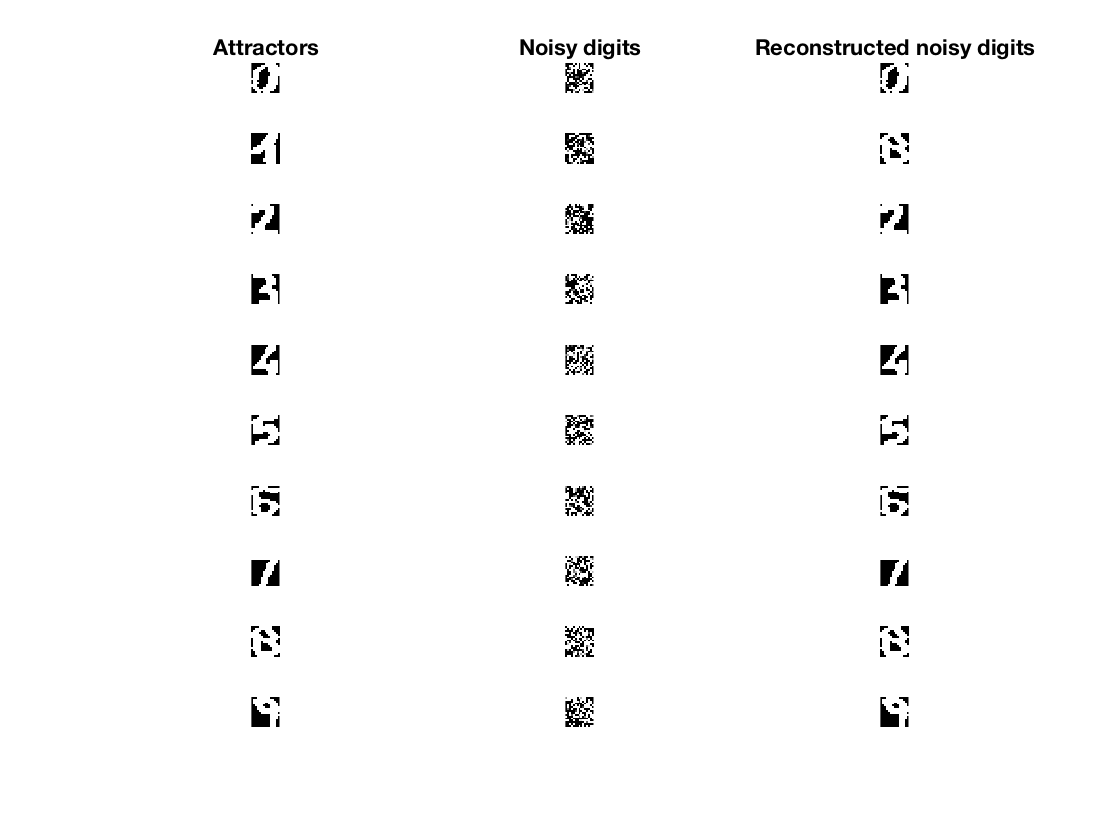
\includegraphics[width=0.8\linewidth]{img/hop5-90}
\end{center}

\begin{center}
	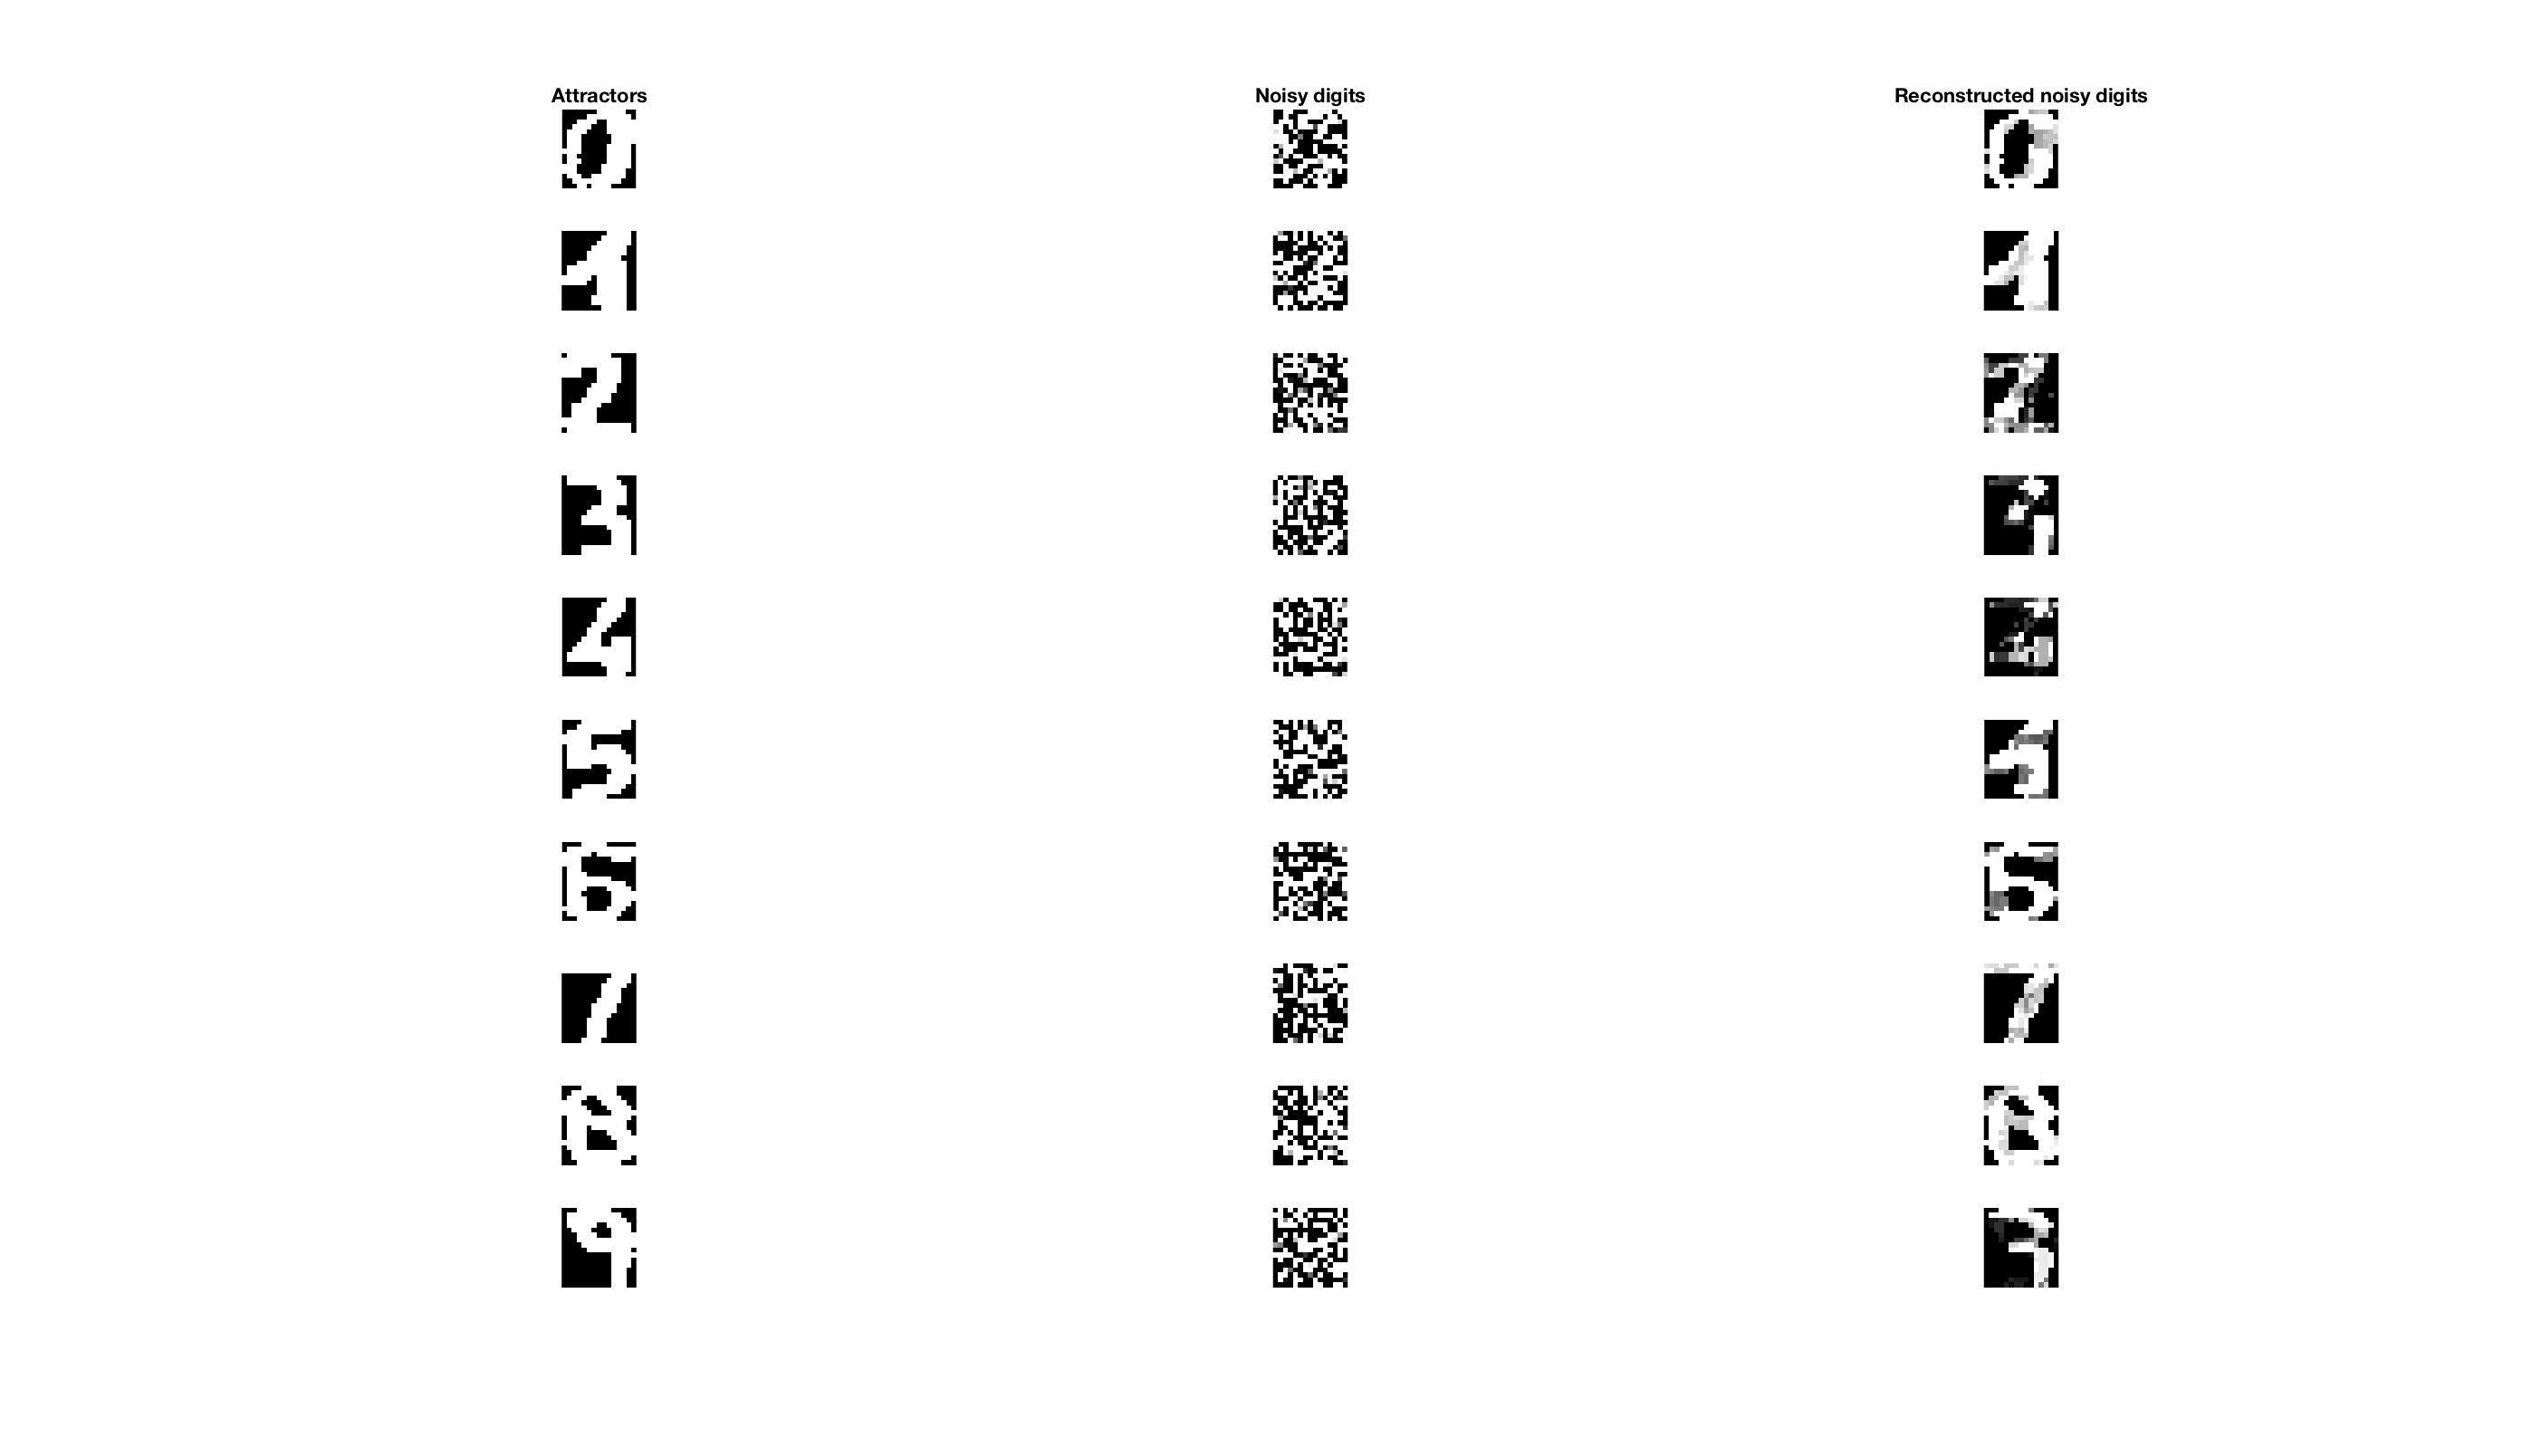
\includegraphics[width=0.8\linewidth]{img/hop6-10}
\end{center}

Although both results contains some incorrect digits, the accuracy of the second image, the one corresponding
with less iterations and more noise, is higher.

The incorrect results are due to the fact that Hopfield networks are guaranteed to converge to a local minimum,
but will sometimes converge to a false pattern (wrong local minimum) rather than the stored pattern (expected local minimum).

\section*{Exercise 2}
With 50 neurons and 500 epochs we obtain the following results:
\begin{center}
	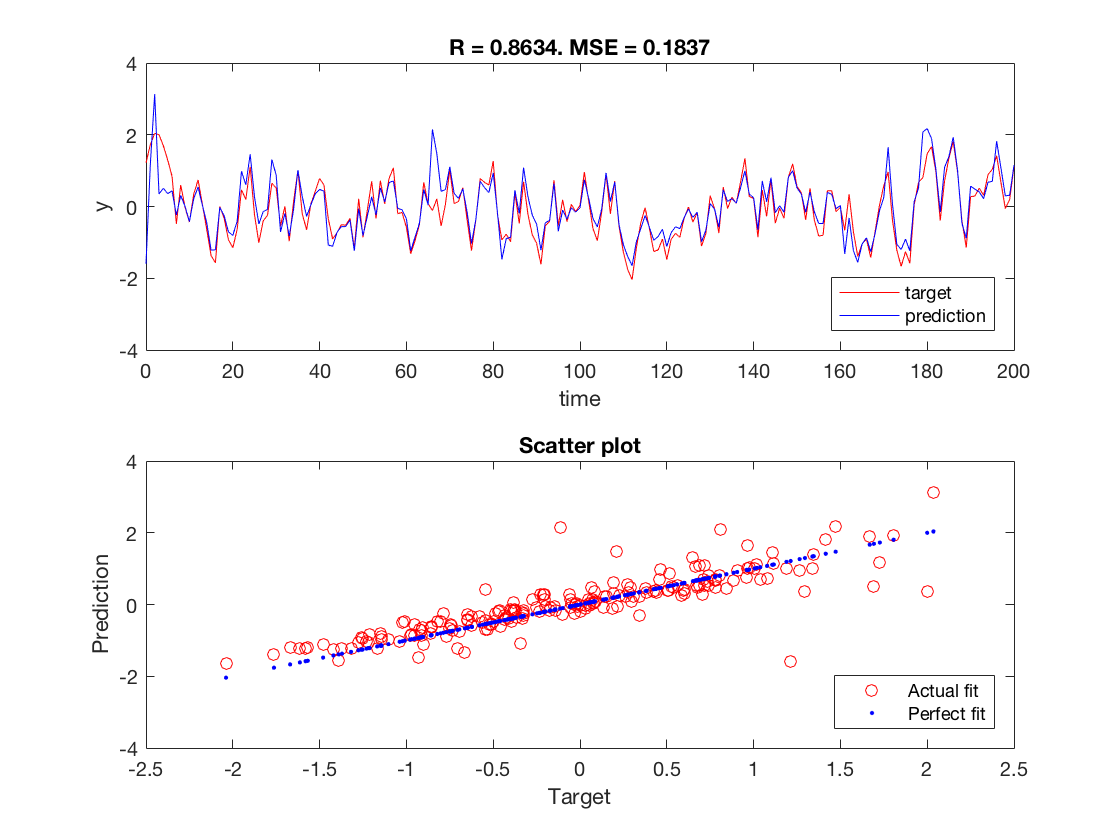
\includegraphics[width=\linewidth]{img/elman1}
\end{center}
It can be seen that the prediction is fairly accurate, with an error of $10^{-1}$. After increasing the number
of training points, the results obtained reamin the same.

The neural network does a good job approximating this time series, and even in those parts in which the approximation
is not exact, it determines when the series increases or decreases almost perfectly.

Increasing the number of neurons does not help either to obtain a more accurate approximation, but to increase the time it takes to
compute the model.

This problem have also been tested with a lower number of neurons, as 50 could be to high. Surprisingly, reducing the number of neurons
to 5, 3 and 1 returns the same results as with 50 neurons.

The number of epochs has been also reduced to 200, giving results as accurate as with 500. This paramter tuning shows that
determining the correct parameters (neurons, epochs, trainign set...) is a difficult task.

\end{multicols}
\end{document}
